\chapter{O simulador}
\label{char:ferrdesenvolvida}
Esse capítulo descreve o \textbf{CryptoEdu - simulador de algoritmos de criptografia com finalidade educacional} criado no decorrer da escrita desse trabalho de conclusão de curso.

O simulador permite a execução completa e passo a passo de todas as etapas envolvidas tanto na criptografia quando na descriptografia utilizando o algoritimo \acrfull{sdes}, escolhido por ser um algoritmo mais recomendado para ensino, como explicado na seção \ref{sec:sdes}.

O público alvo da ferramenta é o corpo docente e discente de cursos de TI. Mas também, pode ser utilizada por todos que desejam aprender como a criptografia de cifra de blocos funcionada, refinar e/ou lapidar os conhecimentos já adquiridos ou até somente desmistificar esse conteúdo complexo chamado criptografia.

\section{Informações técnicas}

O simulador foi desenvolvido na linguagem \textit{Javascript} utilizando \textit{React.js} e \textit{Typescript}. O ambiente de desenvolvimento utilizado foi o \textit{Visual Studio Code}. O código fonte do simulador é \textit{open source} e está disponibilizado no \textit{GitHub} no endereço \textit{https://github.com/TanielianVB/CryptoEdu/}.

No \textit{GitHub} é possível: Gerenciar problemas encontrados e melhorias sugeridas através de \textit{Issues}.; Integrar melhorias implementados por terceiros através de \textit{Pull Requests}.; A publicação de qualquer nova versão está automatizada através da ferramenta \textit{Netlify} (\textit{https://www.netlify.com/}) e reagindo à qualquer nova versão submetida ao repositório. Esses \textit{deploys} podem ser visualizados em \textit{https://app.netlify.com/sites/cryptoedu/deploys/}.; E até, caso necessário, criar uma nova versão do simulador de propriedade de terceiros através do \textit{Fork}.

O simulador está disponibilizado ao usuário através da internet no endereço \textit{https://cryptoedu.netlify.app/}. O simulador pode ser visualizado em \textit{browsers}, inclusive em dispositivos móveis. No entanto a melhor experiência é obtida quando se utiliza uma resolução maior. Normalmente só obtida se utilizando \textit{desktops}.

\section{Estrutura da interface}
Nessa seção são descritos os elementos contidos na interface de maneira estrutural.

\begin{figure}[H]
    \centering
    \caption{Estrutura da interface}
    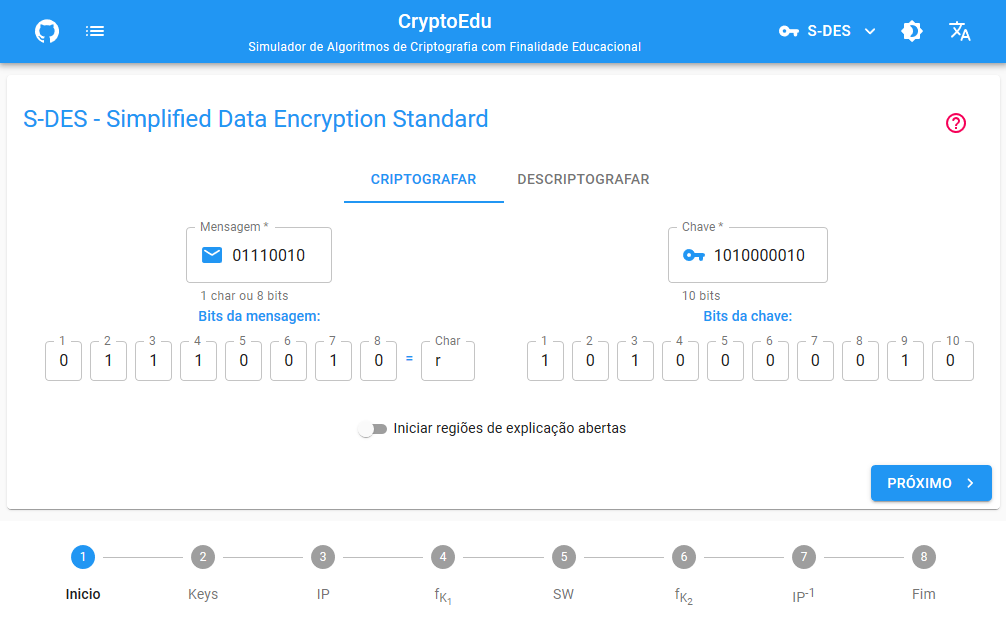
\includegraphics[width=1\linewidth]{UI/UIEstrutura.png}
\end{figure}

\subsection{Cabeçalho}

\begin{figure}[H]
    \centering
    \caption{Cabeçalho}
    
\includegraphics[width=1\linewidth]{UI/UIHeader.png}
\end{figure}

A região do cabeçalho possui:
\begin{itemize}
    \item Link do repositório onde está localizado tanto o código fonte do simulador como um pdf do TCC: \textit{https://github.com/TanielianVB/CryptoEdu}
    \item Link do questionário de \textit{feedback} de utilização do simulador.
    \item O nome do simulador: \textbf{CryptoEdu - Simulador de Algoritmos de Criptografia com Finalidade Educacional}.
    \item \textit{Combo Box} de escolha do algoritmo que está em execução.
    \item Botão para alternar entre o tema \textbf{claro} e \textbf{escuro}.
    \item Botão para alterar o idioma no qual o simulador está sendo exibido.
\end{itemize}

\subsection{Conteúdo}

\begin{figure}[H]
    \centering
    \caption{Conteúdo}
    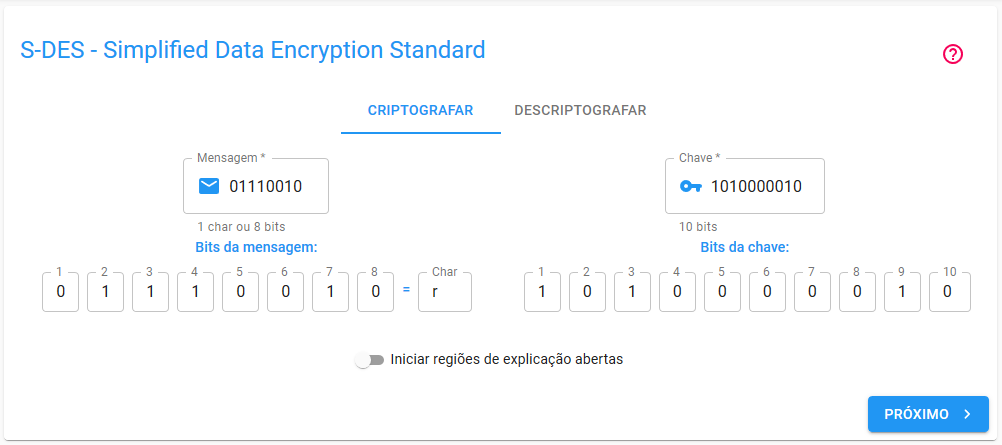
\includegraphics[width=1\linewidth]{UI/UIMain.png}
\end{figure}

A região principal da página será onde cada passo da execução do algoritmo selecionado irá ocorrer. Em cada passo serão listados as etapas executadas em cada passo.

Inicialmente irá conter uma interface discorrendo sobre o algoritmo selecionado e posteriormente cada passo que estará sendo executado. É possível navegar por esses passos através dos botões de navegação (Próximo e Anterior) exibidos na parte inferior da região de cada passo. No último passo o botão Próximo é substituído pelo botão Reiniciar para facilitar o início de uma nova execução.

\subsection{Rodapé}

\begin{figure}[H]
    \centering
    \caption{Rodapé}
    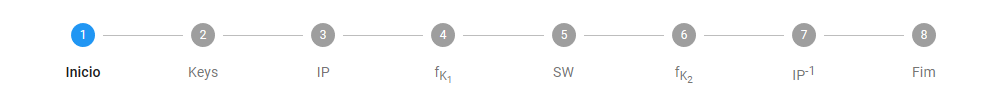
\includegraphics[width=1\linewidth]{UI/UIFooter.png}
\end{figure}

A região do rodapé contém:
\begin{itemize}
    \item Todos os passos necessários para a execução do algoritmo em execução. Ao se passar o mouse sobre eles é exibida uma \textit{tooltip} com um nome mais explicativo do passo.
    \item Quais passos já foram completados.
    \item Qual passo o usuário se encontra no momento.
    \item Quais passos ainda faltam ser completados para finalizar a execução do algoritmo.
\end{itemize}
É possível também, a qualquer momento, navegar para qualquer passo diretamente. Basta-se clicar sobre este.

\subsection{\textit{Mobile}}

\begin{figure}[H]
    \centering
    \caption{Visualização em um \textit{browser} de dispositivo móvel}
    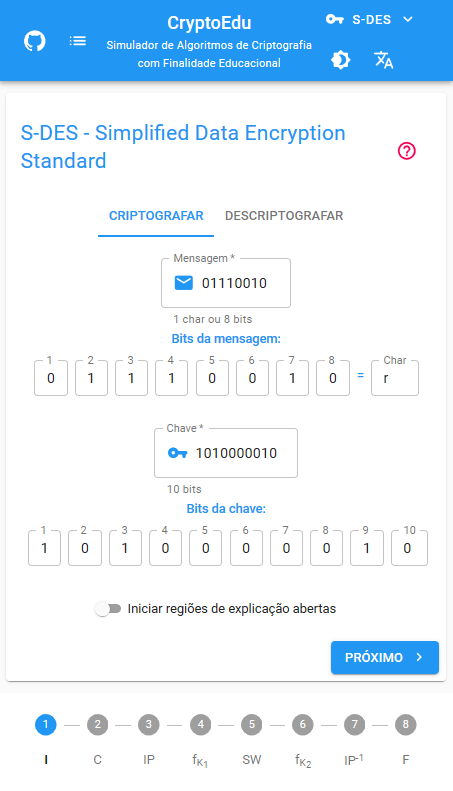
\includegraphics[width=0.5\linewidth]{UI/UIMobile.png}
\end{figure}

Embora não seja o ideal, o simulador se comporta bem em dispositivos móveis melhorando ainda mais a sua acessibilidade.

\section{Interface do conteúdo}
Descrição da interface apresentada em cada um dos passos da execução do algoritmo.

Cada passo possui no mínimo uma etapa e cada etapa possui uma região de explicação onde a etapa é descrita de maneira que possibilite o usuário compreender como a etapa é executada, como essa deve ser compreendida, como esta difere de outras etapas similares e qual a definição matemática desta etapa, caso haja.

A explicação pode ser acessada através do clique do botão interrogação à direita do cabeçalho que contém o título da referida etapa. Esse clique irá expandir a região que contém a explicação da etapa. É possível também que todas as regiões de explicação já iniciem abertas. Basta habilitar a opção \textbf{Iniciar regiões de explicação abertas} ao iniciar a execução da criptografia ou descriptografia.

\subsection{Tela inicial - entrada de dados}

\begin{figure}[H]
    \centering
    \caption{Tela inicial - entrada de dados}
    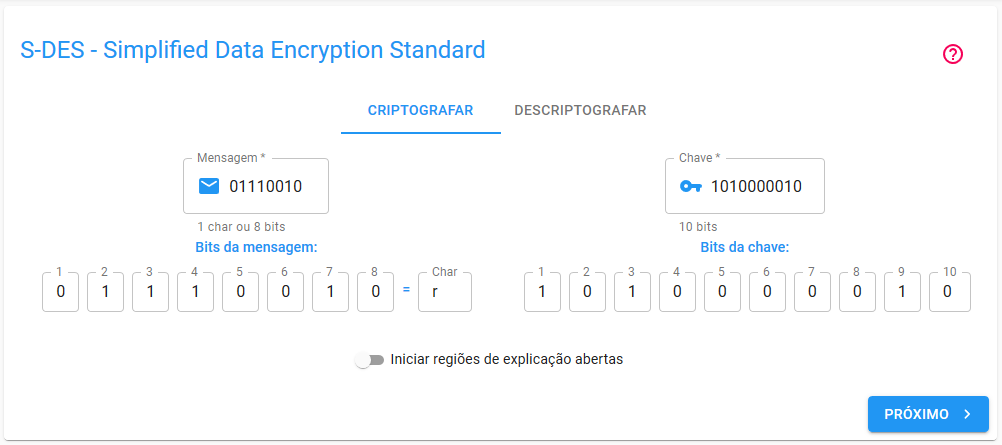
\includegraphics[width=1\linewidth]{UI/UIMain.png}
\end{figure}

A interface inicial faz uma breve descrição do algoritmo selecionado na \textit{Combo Box} de escolha de algoritmo buscando situar o usuário no contexto selecionado para execução. No momento só será disponibilizado um algoritmo: \acrfull{sdes}.

O usuário pode então escolher se ele deseja o fluxo de execução \textbf{criptografar} ou \textbf{descriptografar} e assim então informar valores customizados para os campos \textbf{Mensagem} (\textbf{Mensagem cifrada} caso o fluxo escolhido tenha sido o \textbf{descriptografar}) e \textbf{Chave}.

Os algoritmos recebem como entrada bits. Por conta disso, são exibidos os bits contidos nos campos e que serão utilizados para a execução do fluxo escolhido. Tanto para facilitar o preenchimento do campo \textbf{Mensagem} como para melhorar a compreensão do usuário sobre o valor contido no campo, é possível informar no campo uma letra, visto que essa pode, e é, facilmente convertida para 8 bits. Isso ajuda não somente no preenchimento do campo durante a execução do fluxo \textbf{criptografar} mas também na validação do resultado obtido da execução do fluxo \textbf{descriptografar} visto quê é possível, mais facilmente, comparar as mensagens (tanto a de entrada do fluxo \textbf{criptografar} quando a de saída do fluxo \textbf{descriptografar}) se estas forem letras. Exemplo: A letra \textbf{'T'} gera a sequência de bits: \textbf{01010100}.

Nessa tela também é possível habilitar a opção \textbf{Iniciar regiões de explicação abertas} que fará com que, durante a navegação pelos passos da execução do algoritmo todas as regiões de explicação já se iniciem abertas. Caso o usuário não queria mais visualizar a explicação para alguma etapa. Ele pode esconder a explicação clicando no botão à direita do título da etapa.

\subsection{Passo Chaves - Geração das chaves}

Nesse passo estão concentradas todas as etapas necessárias para a geração das chaves \(K_1\) e \(K_2\). A etapas contidas nesse passo estavam inicialmente divididas em 3 passos. Mas por ter gerado dúvida sobre como essas etapas se relacionavam tanto entre elas como com os outros passos da execução do algoritmo estas etapas estão em um mesmo passo.

\subsubsection{Etapa P10 - Permutação de 10 bits}

\begin{figure}[H]
    \centering
    \caption{Etapa P10 - Permutação de 10 bits}
    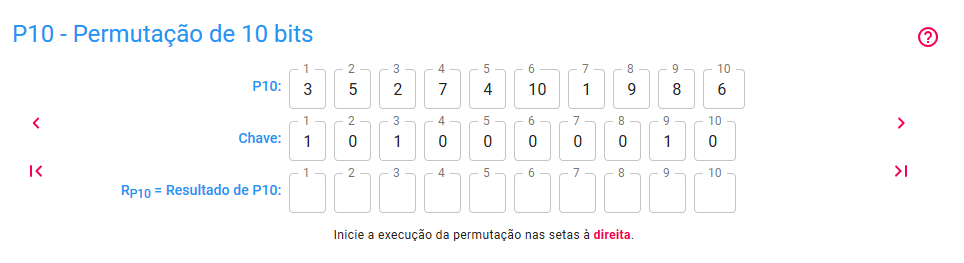
\includegraphics[width=1\linewidth]{UI/UIP10.png}
\end{figure}

A interface da etapa P10 contextualiza o objetivo pelo qual essa etapa existe, explica a definição de uma função de permutação, apresenta a função de permutação P10 (incluindo função matemática) e explica como esta deve ser interpretada. Após tal contextualização se exibe um componente capaz de executar passo a passo a função de permutação P10. O parâmetro de entrada da permutação P10 é a Chave recebida da tela de entrada de dados. O resultado dessa execução será o parâmetro de entrada para a próxima etapa, LS-1.

\subsubsection{Etapa LS-1 - \textit{Circular Left Shift} de 1 posição}

\begin{figure}[H]
    \centering
    \caption{Etapa LS-1 - \textit{Circular Left Shift} de 1 posição}
    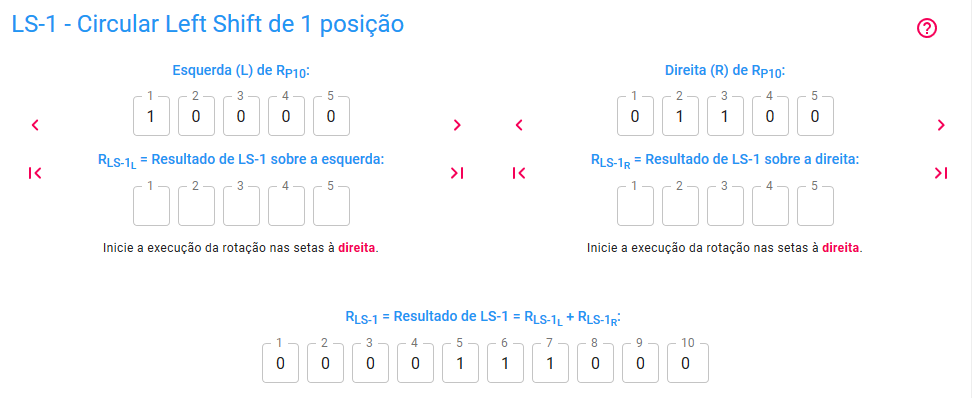
\includegraphics[width=1\linewidth]{UI/UILS1.png}
\end{figure}

A interface da etapa LS-1 contextualiza o objetivo pelo qual essa etapa existe e explica como esta etapa deve ocorrer, incluindo a divisão na metade do valor obtido na etapa anterior (P10) e o que é o processo de rotação. Após tal contextualização se exibe dois componentes capazes de executar passo a passo a rotação circular para a esquerda de 1 posição. Cada um destes componentes irá rotacionar uma das metades. O resultado desta etapa é então a junção das metades após suas rotações individuais.

\subsubsection{Etapa P8 - Permutação de 8 bits sobre o resultado de LS-1}

\begin{figure}[H]
    \centering
    \caption{Passo P8 - Permutação de 8 bits sobre o resultado de LS-1}
    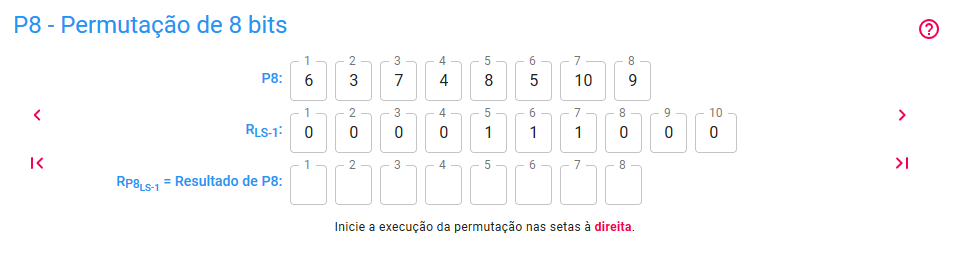
\includegraphics[width=1\linewidth]{UI/UIP81.png}
\end{figure}

A interface da etapa P8 contextualiza o objetivo pelo qual essa etapa existe, explica a definição de uma função de permutação, apresenta a função de permutação P8 (incluindo função matemática) e explica como esta deve ser interpretada. Após tal contextualização se exibe um componente capaz de executar passo a passo a função de permutação P8. O parâmetro de entrada da permutação P8 é o resultado obtido na etapa anterior, LS-1.

\subsubsection{Resultado Chave \(K_1\)}

\begin{figure}[H]
    \centering
    \caption{Chave \(K_1\) - Geração da primeira chave \(K_1\)}
    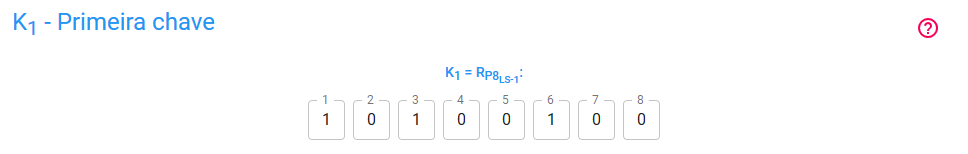
\includegraphics[width=1\linewidth]{UI/UIK1.png}
\end{figure}

O resultado da aplicação da função de permutação P8 sobre o resultado da etapa LS-1 será a primeira chave K1. Esta será utilizada em uma etapa futura durante a criptografia ou descriptografia da mensagem.

\subsubsection{Etapa LS-2 - \textit{Circular Left Shift} de 2 posições}

\begin{figure}[H]
    \centering
    \caption{Etapa LS-2 - \textit{Circular Left Shift} de 2 posições}
    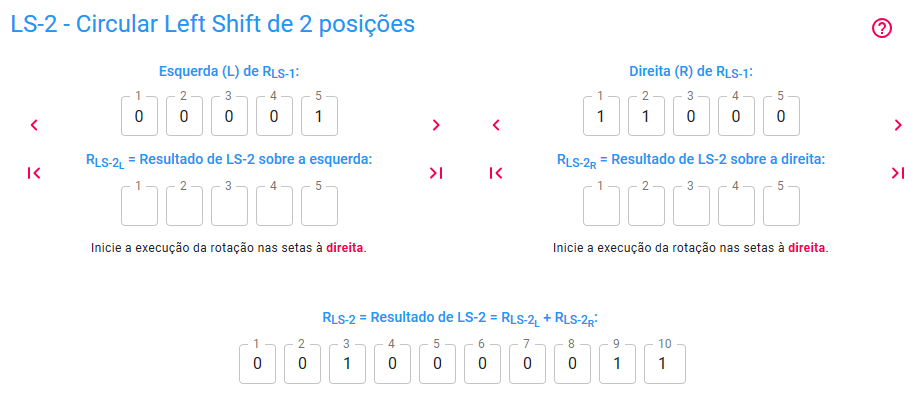
\includegraphics[width=1\linewidth]{UI/UILS2.png}
\end{figure}

A interface da etapa LS-2 contextualiza o objetivo pelo qual essa etapa existe e explica como esta etapa deve ocorrer, incluindo a divisão na metade do valor obtido na etapa LS-1 e o que é o processo de rotação. Após tal contextualização se exibe dois componentes capazes de executar passo a passo a rotação circular para a esquerda de 2 posições. Cada um destes componentes irá rotacionar uma das metades. O resultado desta etapa é então a junção das metades após suas rotações individuais.

\subsubsection{Etapa P8 - Permutação de 8 bits sobre o resultado de LS-2}

\begin{figure}[H]
    \centering
    \caption{Passo P8 - Permutação de 8 bits sobre o resultado de LS-2}
    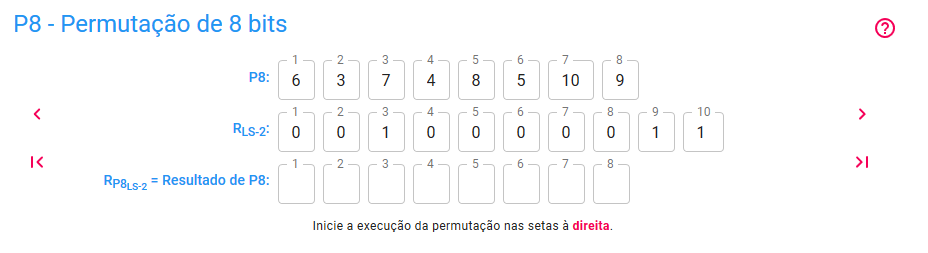
\includegraphics[width=1\linewidth]{UI/UIP82.png}
\end{figure}

A interface da etapa P8 contextualiza o objetivo pelo qual essa etapa existe, explica a definição de uma função de permutação, apresenta a função de permutação P8 (incluindo função matemática) e explica como esta deve ser interpretada. Após tal contextualização se exibe um componente capaz de executar passo a passo a função de permutação P8. O parâmetro de entrada da permutação P8 é o resultado obtido na etapa anterior, LS-2.

\subsubsection{Resultado Chave \(K_2\)}

\begin{figure}[H]
    \centering
    \caption{Chave \(K_2\) - Geração da segunda chave \(K_2\)}
    
\includegraphics[width=1\linewidth]{UI/UIK2.png}
\end{figure}

O resultado da aplicação da função de permutação P8 sobre o resultado da etapa LS-2 será a segunda chave K2. Esta será utilizada em uma etapa futura durante a criptografia ou descriptografia da mensagem.

\subsection{Passo IP - Permutação Inicial}

\begin{figure}[H]
    \centering
    \caption{Passo IP (\textit{Initial Permutation}) - Permutação Inicial}
    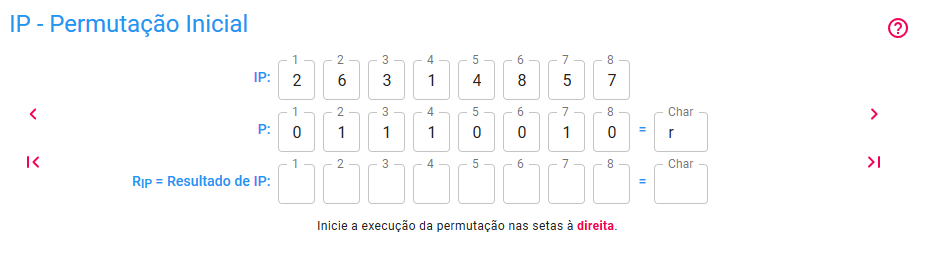
\includegraphics[width=1\linewidth]{UI/UIIP.png}
\end{figure}

A interface da etapa IP contextualiza o objetivo pelo qual essa etapa existe, explica a definição de uma função de permutação, apresenta a função de permutação IP (incluindo função matemática) e explica como esta deve ser interpretada. Após tal contextualização se exibe um componente capaz de executar passo a passo a função de permutação IP. O parâmetro de entrada da permutação IP é a Mensagem (\textit{Plaintext} P) recebida da tela de entrada de dados.

\begin{figure}[H]
    \centering
    \caption{L (esquerda) \& R (direita)}
    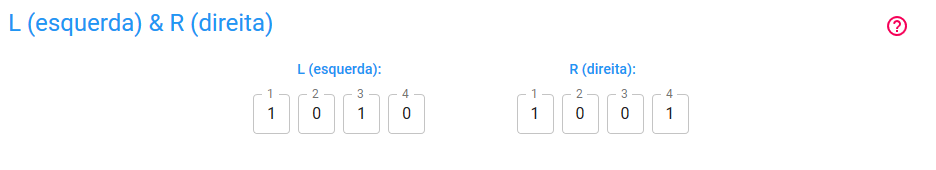
\includegraphics[width=1\linewidth]{UI/UILR.png}
\end{figure}

O resultado desse passo é a divisão do resultado obtido da permutação IP em duas metades, L (\textit{left}) e R (\textit{right}), que serão enfim passados por parâmetro para a execução da função \(f_K\).

\subsection{Passo \(f_K\) - Função que usa uma chave}

\begin{figure}[H]
    \centering
    \caption{Passo \(f_K\) - Função que usa uma chave}
    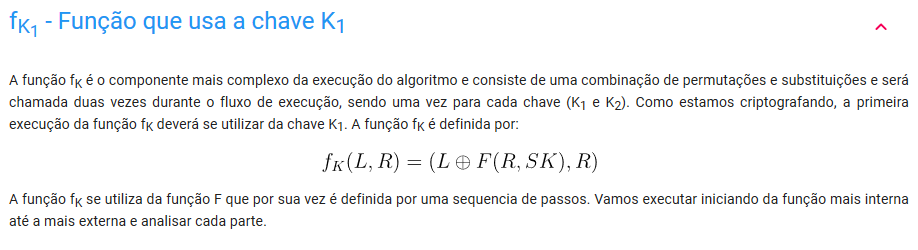
\includegraphics[width=1\linewidth]{UI/UIFK1.png}
\end{figure}

Esse passo é o único passo que se repete durante a execução da criptografia ou descriptografia. Essa função recebe 2 parâmetros de entrada. Um é uma sequência de 8 bits divididos entre L \& R (4 bits na esquerda L e 4 bits na direita R) e o segundo parâmetro é a chave. Caso a execução escolhida seja a criptografia, a primeira vez que essa função é executada a chave utilizada será a \(K_1\) e na segunda vez será a \(K_2\). Caso a execução escolhida seja a descriptografia, a ordem de utilização das chaves será inversa. A interface explica a tais peculiaridades e apresenta a função matemática desta.

Nesse passo estão concentradas todas as etapas da execução da função \(f_K\). A etapas contidas nesse passo estavam inicialmente divididas em 2 passos. Um indo até o primeiro XOR e outro indo até o segundo XOR. Mas por esse passo se repetir optou-se por deixar todas as etapas em um único passo.

\subsubsection{Etapa E/P - Permutação de Expansão}

\begin{figure}[H]
    \centering
    \caption{Etapa E/P - Permutação de Expansão}
    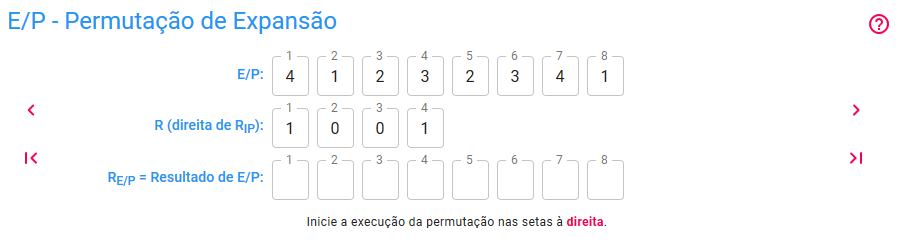
\includegraphics[width=1\linewidth]{UI/UIEP.png}
\end{figure}

A interface da etapa E/P contextualiza o objetivo pelo qual essa etapa existe, explica a definição de uma função de permutação, apresenta a função de permutação E/P (incluindo função matemática) e explica como esta deve ser interpretada. Após tal contextualização se exibe um componente capaz de executar passo a passo a função de permutação E/P. O parâmetro de entrada da permutação E/P é o parâmetro de entrada R da função \(f_K\) (4 bits do lado direito dos 8 bits recebidos de entrada).

\subsubsection{Etapa XOR - OU exclusivo com \(K_1\)}

\begin{figure}[H]
    \centering
    \caption{Etapa XOR - OU exclusivo com \(K_1\)}
    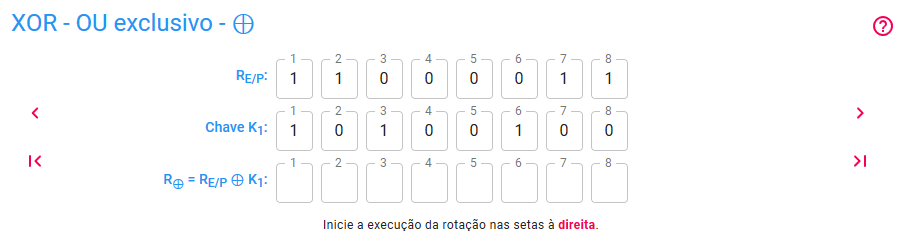
\includegraphics[width=1\linewidth]{UI/UIXORK1.png}
\end{figure}

A interface da primeira etapa XOR descreve o que ocorre nessa etapa e exibe um componente capaz de executar bit a bit a operação XOR (OU exclusivo) para obtenção do resultado dessa etapa. Os parâmetros de entrada dessa etapa são: 1. O resultado da permutação de expansão E/P e 2. Ou a chave \(K_1\) ou a chave \(K_2\). Caso a execução escolhida seja a criptografia, a primeira vez que essa etapa é executada a chave utilizada será a \(K_1\) e na segunda vez será a \(K_2\). Caso a execução escolhida seja a descriptografia, a ordem de utilização das chaves será inversa. A interface reflete essas particularidades em cada fluxo de execução.

\subsubsection{Etapa S0 \& S1 - Substituições S0 e S1}

\begin{figure}[H]
    \centering
    \caption{Etapa S0 \& S1 - Substituições S0 e S1}
    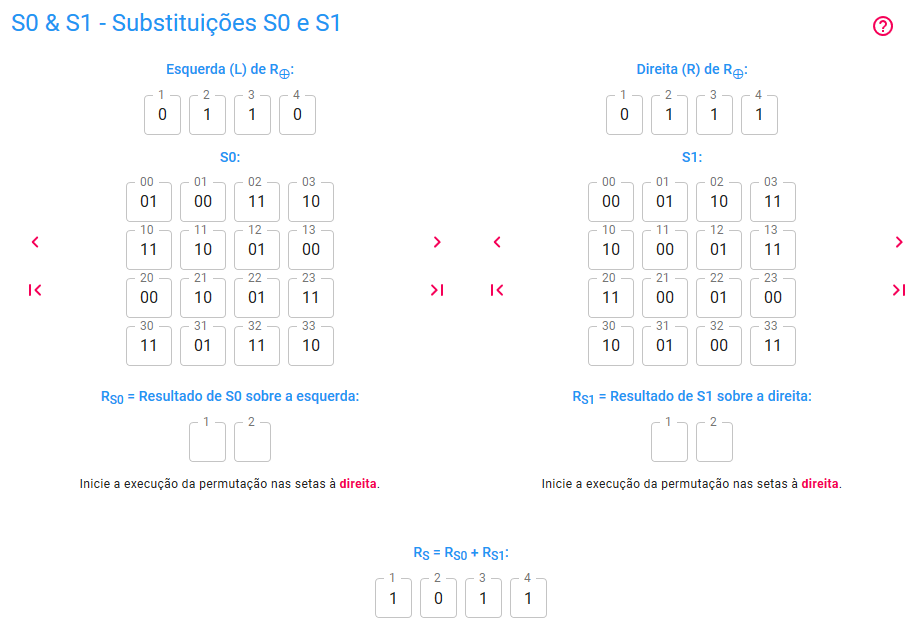
\includegraphics[width=1\linewidth]{UI/UIS0S1.png}
\end{figure}

A interface da etapa das substituições S0 e S1 contextualiza o objetivo pelo qual essa etapa existe, explica a definição de um substituição, apresenta a obtenção dos parâmetros de entrada para cada substituição e explica como uma substituição deve ser interpretada. Após tal contextualização se exibe, para cada substituição, um componente capaz de executar passo a passo a substituição. Os parâmetros de entrada das substituições S0 e S1 são, respectivamente, as metades esquerda e direita do resultado obtido na etapa anterior (XOR com \(K_1\)). O resultado desta etapa é então a junção das metades após suas substituições individuais.

\subsubsection{Etapa P4 - Permutação de 4 bits}

\begin{figure}[H]
    \centering
    \caption{Etapa P4 - Permutação de 4 bits}
    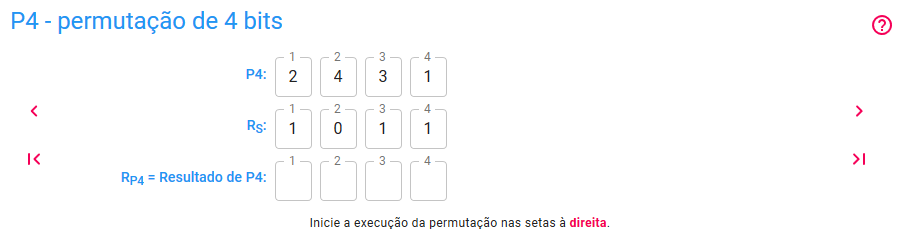
\includegraphics[width=1\linewidth]{UI/UIP4.png}
\end{figure}

A interface da etapa P4 contextualiza o objetivo pelo qual essa etapa existe, explica a definição de uma função de permutação, apresenta a função de permutação P4 (incluindo função matemática) e explica como esta deve ser interpretada. Após tal contextualização se exibe um componente capaz de executar passo a passo a função de permutação P4. O parâmetro de entrada da permutação P4 é o resultado obtido na etapa anterior (Substituições S0 e S1). O resultado dessa execução será o parâmetro de entrada para a próxima etapa, XOR com L.

\subsubsection{Etapa XOR - OU exclusivo com L}

\begin{figure}[H]
    \centering
    \caption{Etapa XOR - OU exclusivo com L}
    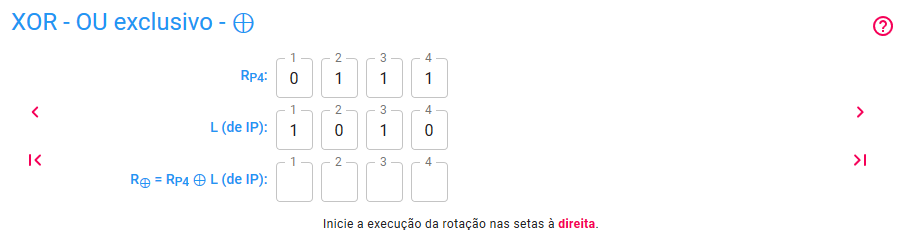
\includegraphics[width=1\linewidth]{UI/UIXORL.png}
\end{figure}

A interface da segunda etapa XOR descreve o que ocorre nessa etapa e exibe um componente capaz de executar bit a abit a operação XOR (OU exclusivo) para obtenção do resultado dessa etapa. Os parâmetros de entrada dessa etapa são: 1. O resultado da permutação P4 e 2. L (metade esquerda do parâmetro de entrada de \(f_K\)). Na primeira vez que \(f_K\) é executada L será a esquerda do resultado da permutação inicial (IP) e na segunda vez L será a esquerda do resulta da Troca (SW).

\subsubsection{Resultado de \(f_K\)}

\begin{figure}[H]
    \centering
    \caption{Resultado de \(f_K\)}
    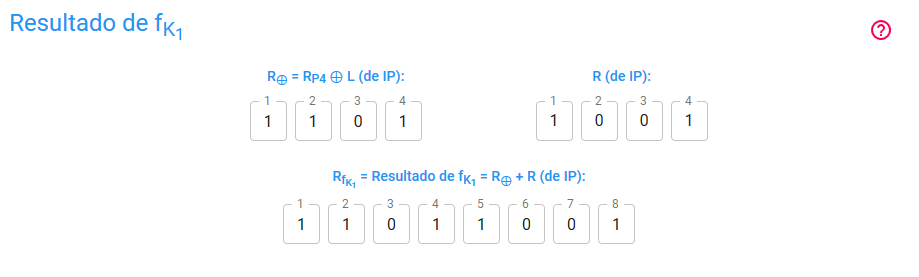
\includegraphics[width=1\linewidth]{UI/UIRFK1.png}
\end{figure}

A interface do resultado de \(f_K\) exibe as metades que compõem o resultado da função e a junção destes. A metade esquerda desse resultado sempre será o resultado da etapa anterior, XOR. A metade direita será a metade direita do parâmetro de entrada da função \(f_K\). Que na primeira vez é a metade direita do resultado da permutação inicial (IP) e na segunda vez é a matade direita da Troca (SW).

\subsection{Passo SW - Troca}

\begin{figure}[H]
    \centering
    \caption{Passo SW - Troca}
    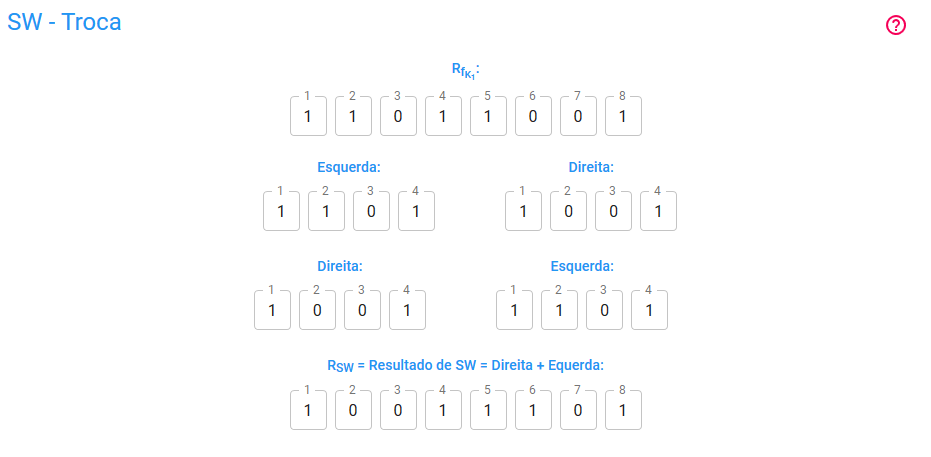
\includegraphics[width=1\linewidth]{UI/UISW.png}
\end{figure}

A interface do passo Troca (SW) explica a definição da troca, apresenta a função de troca (incluindo função matemática) e explica como esta deve ser interpretada. Este é o passo intermediário entre as execuções das funções \(f_K\). Ela recebe por parâmetro o resultado da primeira execução da função \(f_K\) e o resultado deste passo é o parâmetro de entrada para a segunda execução da função \(f_K\) juntamente com a chave que não foi utilizada pela primeira execução.

\subsection{Passo \(f_K\) - Função que usa a outra chave}

A segunda execução da função \(f_K\) é sequencialmente idêntica à primeira logo as interfaces de cada etapa são similares. As únicas diferenças são:
\begin{itemize}
    \item O parâmetro de entrada é o resultado do passo Troca (SW) e não o resultado do passo Permutação inicial (IP) como ocorre na primeira execução da função.
    \item A chave utilizada é a chave que não foi utilizada na primeira execução da função \(f_K\). Na criptografia a primeira execução da função \(f_K\) utiliza a chave \(K_1\) e a segunda execução a chave \(K_2\). Já na descriptografia o inverso é verdade. A interface identifica o fluxo que está sendo executado e reflete essas diferenças tanto nas \textit{labels} quanto nas explicações das etapas.
\end{itemize}

\subsection{Passo \(IP^{-1}\) - Permutação Inicial Inversa}

\begin{figure}[H]
    \centering
    \caption{Passo \(IP^{-1}\) - Permutação Inicial Inversa}
    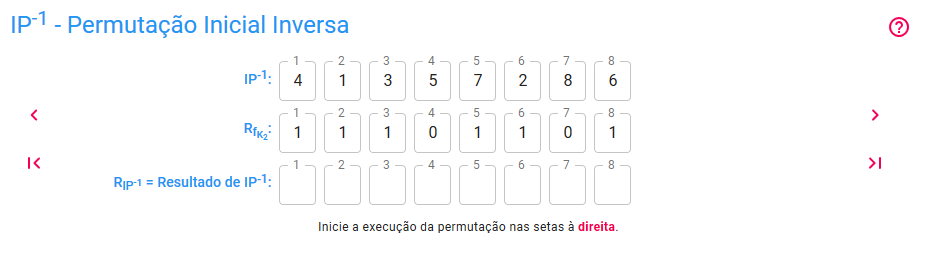
\includegraphics[width=1\linewidth]{UI/UIIP-1.png}
\end{figure}

A interface da etapa \(IP^{-1}\) contextualiza o objetivo pelo qual essa etapa existe, explica a definição de uma função de permutação, apresenta a função de permutação \(IP^{-1}\) (incluindo função matemática) e explica como esta deve ser interpretada. Após tal contextualização se exibe um componente capaz de executar passo a passo a função de permutação \(IP^{-1}\). O parâmetro de entrada da permutação \(IP^{-1}\) é o resultado obtido no passo anterior (\(f_K\)).

\subsection{Tela final - Resultado}

\begin{figure}[H]
    \centering
    \caption{Resultado}
    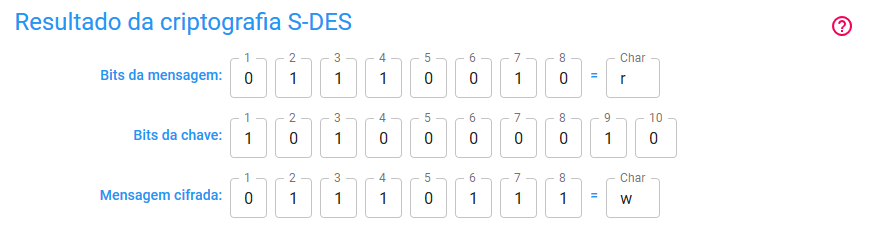
\includegraphics[width=1\linewidth]{UI/UIResult.png}
\end{figure}

A interface do último passo exibe os dois parâmetros de entrada da execução, a Mensagem e a Chave, e o resultado da execução da criptografia ou descriptografia.

\begin{figure}[H]
    \centering
    \caption{\textit{Feedback request}}
    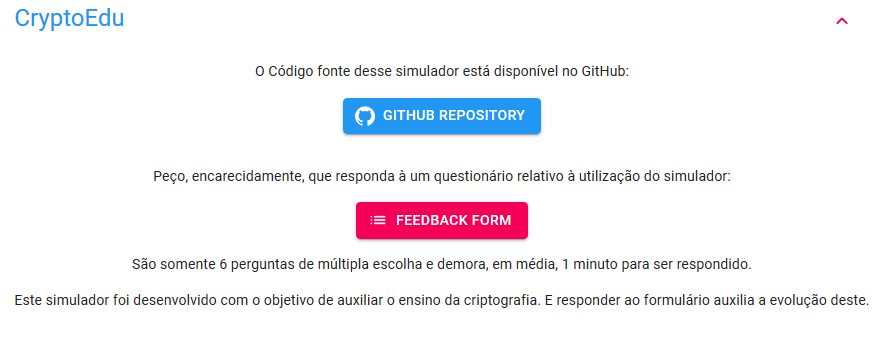
\includegraphics[width=1\linewidth]{UI/UIFeedback.png}
\end{figure}

O último ponto na interface é uma solicitação do preenchimento do questionário de utilização do simulador. É exibido também um link para o repositório \textit{GitHub} onde se encontra o simulador. No \textit{GitHub} também é possível baixar a última versão publicada deste \acrshort{tcc}.

\section{Limites da solução}
A ferramenta foi desenvolvida prevendo uma fácil extensão das suas atuais funcionalidades. Mas, visto que o escopo do projeto pode, facilmente, se exceder além do limite possível de execução de um trabalho de conclusão de curso, alguns limites foram impostos para viabilizar o desenvolvimento da ferramenta em tempo hábil. São eles:
\begin{itemize}
    \item Somente 1 algoritmo será disponibilizado. Sendo este, o \acrfull{sdes}.
    \item Só estará disponibilizado no tema \textbf{claro}.
    \item Só estará disponibilizado em \textbf{Português-BR}.
    \item A interface terá foco para dispositivos \textit{desktop}.
\end{itemize}

\section{Comparação com outros simuladores criptográficos}
Os simuladores foram comparados em alguns pontos: \textbf{Idioma}; \textbf{Algoritmos}, quais algoritmos o simulador é capaz de simular; \textbf{Educativo}, se o simulador é voltado ao ensino ou não; \textbf{I/O}, nível de detalhamento das entradas e saídas, em que, \textbf{algoritmo} exibe somente as entradas e saídas do algoritmo, \textbf{passo} exibe também as entradas e saídas de cada passo do algoritmo e \textbf{etapa} exibe também as entradas e saídas de cada etapa dentro de cada passo; \textbf{\textit{Open Source}}, se o simulador possui código aberto e permite ou não que colaboradores extendam suas funcionalidades; \textbf{Plataforma}; e \textbf{Responsivo}, que indica o nível de responsividade da interface do simulador.

Comparando o simulador desenvolvido com os outros simuladores criptográficos encontrados, levando em consideração os pontos já explícitos, temos:

\begin{table}[h!]
\centering
    \addtolength{\leftskip} {-3cm} % increase (absolute) value if needed
    \addtolength{\rightskip}{-2cm}
\resizebox{1.2\textwidth}{!}{%
\begin{tabular}{ c | c c c c c c }
 \xrowht{20pt} & \textbf{CyberChef} & \textbf{CrypTool} & \textbf{S-DES Sim. App} & \textbf{S-DES Sim. \textit{online}} & \textbf{S-DES Sim. Win} & \textbf{CryptoEdu} \\
 \hline
 \xrowht{20pt} \textbf{Idioma} & Inglês & Inglês & Inglês & Koreano & Inglês & \cellcolor{green!70!yellow!40} Português \\
 \xrowht{20pt} \textbf{Algoritmos} & Vários & Vários & \cellcolor{green!70!yellow!40} S-DES & \cellcolor{green!70!yellow!40} S-DES & \cellcolor{green!70!yellow!40} S-DES & \cellcolor{green!70!yellow!40} S-DES \\
 \xrowht{20pt} \textbf{Educativo} & Não & \cellcolor{green!70!yellow!40} Sim & \cellcolor{green!70!yellow!40} Sim & \cellcolor{green!70!yellow!40} Sim & \cellcolor{green!70!yellow!40} Sim & \cellcolor{green!70!yellow!40} Sim \\
 \xrowht{20pt} \textbf{I/O} & algoritmo & algoritmo & passo & passo & passo & \cellcolor{green!70!yellow!40} etapa \\
 \xrowht{20pt} \textbf{\textit{Open Source}} & \cellcolor{green!70!yellow!40} Sim & Não & Não & \cellcolor{green!70!yellow!40} Sim & Não & \cellcolor{green!70!yellow!40} Sim \\
 \xrowht{20pt} \textbf{Plataforma} & \cellcolor{green!70!yellow!40} \textit{online} & SO's & Android & \cellcolor{green!70!yellow!40} \textit{online} & Windows & \cellcolor{green!70!yellow!40} \textit{online} \\
 \xrowht{20pt} \textbf{Responsivo} & \textit{desktop} & \textit{desktop} & \cellcolor{green!70!yellow!40} \textit{mobile} & \textit{desktop} & \textit{desktop} & \cellcolor{green!70!yellow!40} \textit{desktop} e \textit{mobile} \\
\end{tabular}}
\end{table}

Foram marcados de verde, na tabela, os pontos dos simuladores que se sobressaem quando analisados em um contexto de acessibilidade e ensino-aprendizagem.

%\begin{itemize}
    %\item É mais acessível. Somente 2 dos outros simuladores estão \textit{online}, nenhum deles é utilizável em \textit{mobile}, destes somente 1 é voltado para o ensino e este está em Koreano. 
    %\item Possui detalhamento da execução do algoritmo. Embora alguns outros simuladores sejam voltados ao ensino, nenhum deles explica o processo que ocorre dentro das etapas do algoritmo muito menos permite uma execução passo a passo dos processos contidos nessas etapas.
%\end{itemize}
